

%-------------------------------------------------------------------------------
% Dokumenten Klasse
\documentclass[
	final,
	a4paper,
	oneside,
	parskip=full,
	headings=standardclasses,
	headings=big,
	pointednumbers
]{scrartcl}

%-------------------------------------------------------------------------------
% Packete nutzen
\usepackage{ngerman,palatino,setspace}
\usepackage[T1]{fontenc}
\usepackage[latin9]{inputenc}
\usepackage[left=35mm,right=35mm,top=25mm,bottom=25mm]{geometry}
\usepackage{graphicx}
\usepackage{scrpage2}
\usepackage{listings}
\usepackage[usenames,dvipsnames,svgnames]{xcolor}
\usepackage[hidelinks]{hyperref}
\usepackage{amsmath}
\usepackage{caption}

%-------------------------------------------------------------------------------
% Kopf- und Fusszeile

\pagestyle{scrheadings}
\clearscrheadfoot
\chead{Projekt 1: Implizite Euler und Trapezmethode}
\cfoot[Seite \thepage]{Seite \thepage}

%-------------------------------------------------------------------------------
%
\title{Projekt 1: Implizite Euler und Trapezmethode}
\subtitle{MND2}
\author{Andreas Bachmann \\ \href{mailto:bachman0@students.zhaw.ch}{bachman0@students.zhaw.ch}}
\date{\today}

%-------------------------------------------------------------------------------
% Dokumenten Einstellungen

% Section Abst�nde
\RedeclareSectionCommand[
	beforeskip=-1\baselineskip,
	afterskip=0.001\baselineskip
]{section}
\RedeclareSectionCommand[
	beforeskip=0\baselineskip,
	afterskip=0.001\baselineskip
]{subsection}

% Formeln
\DeclareCaptionType{mycapequ}[aa][bb]
\captionsetup[mycapequ]{labelformat=empty}

%-------------------------------------------------------------------------------
% Listings

\newcommand{\listingMatlab}[2][]{
	\lstset{
		language=Matlab,
		breaklines=true,
		numbers=left,
		numberstyle=\tiny,
		numbersep=5pt,
		captionpos=b,
		basicstyle=\footnotesize\ttfamily,
		stringstyle=\color{magenta},
		identifierstyle=\color{black},
		keywordstyle=\color{blue}, 
		commentstyle=\color{DarkGreen}
	}
	\lstinputlisting[caption={\texttt{\detokenize{#2}}},#1]{#2}
}

%-------------------------------------------------------------------------------
% Dokument
\begin{document}
	\maketitle
	\section*{Einf�hrung}
	Gesucht ist die L�sung des nichtlinearen Anfangswertproblems:
	\begin{align*}
		x & \in \left( 0, 4 \pi \right] \\
		y' \left( x \right) & = \cos \left( y \left( x \right) \right) + \sin \left( x \right) \\
		y \left( 0 \right) & =-1
	\end{align*}
	\vspace{-1.5cm}
	
	\section*{Aufgabe 1}
	Berechnen Sie mit Hilfe der Methode nach Runge numerisch eine L�sung der DGL.
	
	\subsection*{L�sung}

	\listingMatlab[frame=single]{aufgabe1.m}
	
	
	%\vspace{-1.0cm}
	\begin{mycapequ}[!ht]
		\begin{align*}
			r_{1}   & = f \left( x_{k}, \; y_{k} \right) \\
			r_{2}   & = f \left( x_{k} + \frac{h}{2}, \; y_{k} + \frac{h}{2} \cdot r_{1} \right) \\
			y_{k+1} & = y_{k} + h \cdot r_{2}
		\end{align*}
		\vspace{-0.75cm}
		\caption{Algorithmus}
	\end{mycapequ}
	
	\listingMatlab[frame=single]{explicitRunge.m}
	
	
	\begin{figure}[htbp] 
		\centering
		\includegraphics[width=0.7\textwidth]{aufgabe1.eps}
		\vspace{-10pt}
		\caption{Explizites Runge-Verfahreb}
		\label{fig:runge}
	\end{figure}
	
	\newpage
	
	\section*{Aufgabe 2}
	Notieren Sie die nichtlineare Gleichung f�r das \textbf{implizite Eulerverfahren}.
	Die Gleichung ist analytisch nicht nach $ y_{n+1} $ aufl�sbar.
	
	\subsection*{L�sung}
	
	Nichtlineare Gleichung f�r das implizite Eulerverfahren
	\begin{align*}
		f\left(x, \; y\right) & =y'\left(x\right)=\cos\left(y\left(x\right)\right)+\sin\left(x\right)\\
		y_{k+1} & = y_k + h \cdot f\left(x_{k+1}, \; y_{k+1}\right)
	\end{align*}
	\vspace{-0.75cm}

	Newton-Verfahren
	\begin{align*}
		y_{k+1}                & = y_k   + h \cdot f\left(x_{k+1}, y_{k+1}\right)\\
		s                      & = y_k   + h \cdot f\left(x_{k+1}, s\right)\\
		0                      & = s-y_k - h \cdot f\left(x_{k+1}, s\right)\\
		G\left(s\right)        & = s-y_k - h \cdot f\left(x_{k+1}, s\right) = 0 \\
		s^{\left( n+1 \right)} & = s^{ \left( n \right) } - \frac{G \left( s^{ \left( n \right) } \right)}
                                                        {G' \left(s^{\left(n\right)} \right) } \\
		s^{\left(n\right)}     & \to s^{\left(\text{Iterationsschritt}\right)}
	\end{align*}
	\vspace{-0.75cm}

	Einsetzen der Funktion
	\begin{align*}
		f\left(x, y\right) & = \cos\left(y\right)+\sin\left(x\right)\\
		G\left(s\right)    & = s-y_k - h \cdot f\left(x_{k+1}, s\right)\\
		G\left(s\right)    & = s-y_k - h \cdot \left[ \cos\left(s\right)+\sin\left(x_{k+1}\right) \right]\\
		G\left(s\right)    & = s-y_k - h \cdot \cos\left(s\right) - h \cdot \sin\left(x_{k+1}\right)
	\end{align*}
	\vspace{-0.75cm}
	
	$ G'\left(s\right) $ ableiten
	\begin{lstlisting}[frame=single]
syms s yk h xkp1
g = s - yk - h*cos(s) - h*sin(xkp1)
diff(g,s)
% h*sin(s) + 1
	\end{lstlisting}
	
	
	
	Einsetzen der Funktion
	\begin{align*}
		G\left(s\right)          & = s-y_k - h \cdot \cos\left(s\right) - h \cdot \sin\left(x_{k+1}\right)\\	
		G'\left(s\right)         & = \frac{dG}{ds} = h \cdot \sin\left(s\right) + 1\\
		s^{ \left( n+1 \right) } & = s^{ \left( n \right) } - \frac{G \left( s^{ \left( n \right) } \right) } 
		                                                           {G'\left( s^{ \left( n \right) } \right) } \\
		s^{ \left( n+1 \right) } & = s^{ \left( n \right) } - \frac{s^{\left(n\right)} - y_k - h \cdot \cos\left(s^{\left(n\right)}\right) - h \cdot \sin\left(x_{k+1}\right)}
		{h \cdot \sin\left(s^{\left(n \right)} \right) + 1}
	\end{align*}

	
	\section*{Aufgabe 3}
	Setzen Sie den folgenden Algorithmus um
	
	\listingMatlab[frame=single]{aufgabe3.m}
	
	\listingMatlab[frame=single]{implizitEulerNewton.m}
	
	\listingMatlab[frame=single]{newton.m}
	
	
	\begin{figure}[htbp] 
		\centering
		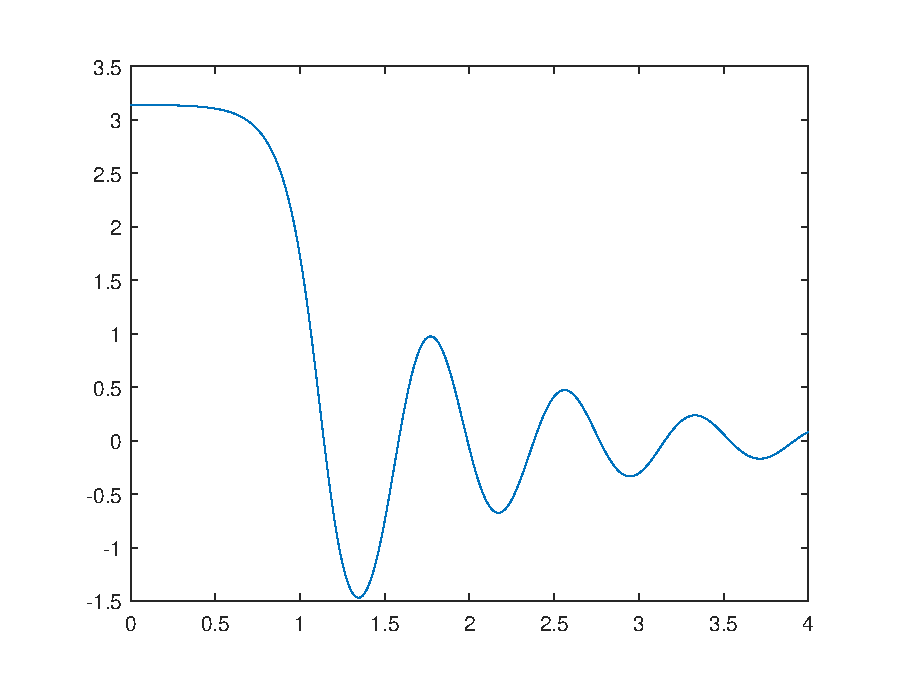
\includegraphics[width=0.7\textwidth]{aufgabe3.eps}
		\vspace{-10pt}
		\caption{Implizites Euler-Verfahren}
		\label{fig:euler}
	\end{figure}
	
	
	\section*{Aufgabe 4}
	Wenden Sie die Methode auf die \textbf{implizite Trapezmethode} an.
	
	\subsection*{L�sung}
	
	\listingMatlab[frame=single]{aufgabe4.m}
	
	\listingMatlab[frame=single]{implicitTrapez.m}
	
	\begin{figure}[htbp] 
		\centering
		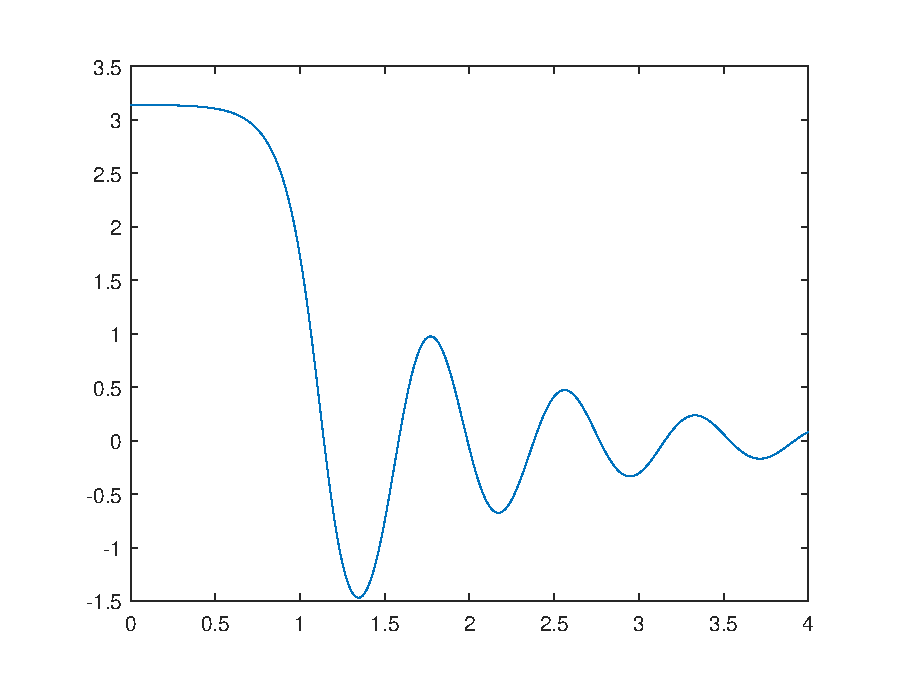
\includegraphics[width=0.7\textwidth]{aufgabe3.eps}
		\vspace{-10pt}
		\caption{Implizite Trapezmethode}
		\label{fig:trapez}
	\end{figure}
	
	
	\newpage
	
	\section*{Aufgabe 5}
	Vergleichen Sie die drei verschiedenen L�sungen mit Hilfe einer Referenzl�sung, f�r
	welche Sie eine 10x kleinere Schrittweite h verwenden.
	
	\subsection*{L�sung}
	
	\listingMatlab[frame=single]{aufgabe5.m}
	
	\begin{figure}[htbp] 
		\centering
		\includegraphics[width=0.7\textwidth]{aufgabe5.eps}
		\vspace{-10pt}
		\caption{Vergleich}
		\label{fig:vergleich}
	\end{figure}

	\section*{Aufgabe 6}
	Leiten Sie die linearisierte DGL her und l�sen Sie diese mit Hilfe der impliziten
	Trapezmethode. Vergleichen Sie die L�sung mit der L�sung aus Schritt 4.
	
	\subsection*{L�sung}
	
	\listingMatlab[frame=single]{aufgabe6.m}
	
	\begin{figure}[htbp] 
		\centering
		\includegraphics[width=0.7\textwidth]{aufgabe6.eps}
		\vspace{-10pt}
		\caption{Vergleich mit Linear}
		\label{fig:vergleich2}
	\end{figure}
	
	\newpage
	
	\section*{Aufgabe 7}
	Leiten Sie die DGL mit einer Reihenentwicklung bis zum quadratischen Term her
	und l�sen Sie diese mit Hilfe der impliziten Trapezmethode. Vergleichen Sie die L�sung
	wiederum mit der L�sung aus Schritt 4. (Die Verfahrensformel kann analytisch
	berechnet werden.)
	
	\subsection*{L�sung}
		\begin{mycapequ}[!ht]
		\begin{align*}
		T_{\infty, \; x_{0}} f \left(x\right)   & = \sum_{k=0}^\infty \frac{f^{\left(k\right)} \left(x_{0}\right)}{k!}
		                                             \left( x - x_{0} \right)^k\\
		f \left( y \right)                      & = \cos \left( y \right) \\
		T_{2, \; 0} f \left(y\right)            & = \cos \left( 0 \right) - \sin \left( 0 \right) \cdot y -
		                                            \frac{\cos \left( 0 \right)}{2!} \cdot y^{2}\\
		                                        & = 1 - \frac{1}{2} \cdot y^{2}\\
		y' \left( x \right)                     & = f \left( x, \; y \right)\\
		y' \left( x \right)                     & = 1 - \frac{1}{2} \cdot y^{2} + \sin \left( x \right)
		\end{align*}
		\caption{Algorithmus}
	\end{mycapequ}

	\newpage

	\listingMatlab[frame=single]{aufgabe7.m}
	
	\begin{figure}[htbp] 
		\centering
		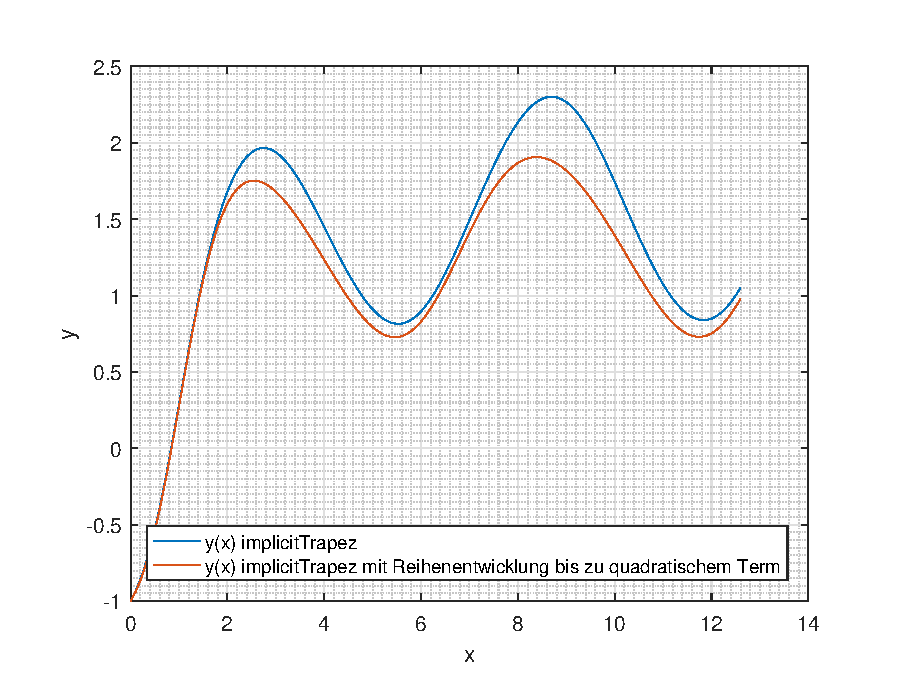
\includegraphics[width=0.7\textwidth]{aufgabe7.eps}
		\vspace{-10pt}
		\caption{Vergleich mit Reihenentwicklung}
		\label{fig:vergleich2}
	\end{figure}
		
\end{document}